% # COPYRIGHT:
%
% Copyright (C) 2011 Jeremiah Mahler <jmmahler@gmail.com>.
% Permission is granted to copy, distribute and/or modify this document
% under the terms of the GNU Free Documentation License, Version 1.3
% or any later version published by the Free Software Foundation;
% with no Invariant Sections, no Front-Cover Texts, and no Back-Cover Texts.
% A copy of the license is included in the file "fdl-1.3.txt".
%
\documentclass[12pt]{article}
%\usepackage{mslapa}
\usepackage{hyperref}
\usepackage{amsmath}
\usepackage{graphicx}
\usepackage{ulem}
\usepackage{vmargin}
\usepackage{tabularx}
\usepackage{sectsty}
\usepackage{pbox}
\usepackage{bigstrut}
\usepackage{enumerate}
\usepackage{parskip} % add spaces between paragraphs
\input kvmacros % Karnaugh Maps and Veitch charts
%\usepackage{cleveref}
\usepackage{verbatim}
\usepackage{listings}

\setpapersize{USletter}
\setmarginsrb{1.0in}{1.0in}{1.0in}{1.0in}{0in}{0.25in}{0in}{0.20in}

\sectionfont{\normalsize}
\subsectionfont{\normalsize}

% configure \bigstrut size
% This configures spacing above and below rows in a tabularx.
%\renewcommand{\bigstrutjot}{6pt}

\renewcommand{\bigstrutjot}{2.0\jot}

\setlength{\parindent}{0in}

\raggedright

\begin{document}

% {{{ Cover Page
\centerline{\bf EECE 144}
\centerline{\bf Fall 2011}
\centerline{\bf}
\centerline{\bf Lab Report \#12}
\centerline{\bf Section 4}
\centerline{\bf 11/30/2011} % date due
% signature area
\begin{center}
\begin{tabularx}{\textwidth}[b]{X l l}
Submitted by: Jeremiah Mahler & & \\
Signature & Printed Name & Date \\
\hline
\multicolumn{1}{|X|}{} & \multicolumn{1}{|l|}{\bigstrut \bf Jeremiah Mahler} & \multicolumn{1}{|l|}{\bf Nov 30, 2011} \\
\hline
\multicolumn{1}{|X|}{} & \multicolumn{1}{|l|}{\bigstrut \bf Marvanee Johnson} & \multicolumn{1}{|l|}{\bf Nov 30, 2011} \\
\hline
\end{tabularx}
\end{center}
% }}}

% {{{ Description/Objectives
\section{Description/Objectives}

The objective of this lab is to implement the three bit non-sequential
counter from Lab 11\cite{mahler144lab11} in Verilog along with
an additional synchronous reset input.
The counter will count in ascending order from top to
bottom when $X = 0$ and in reverse order when $X = 1$.

\begin{center}
\begin{tabular}[t]{cccc}
0 & 0 & 0 \\
0 & 1 & 0 \\
1 & 1 & 0 \\
0 & 1 & 1 \\
1 & 0 & 1 \\
0 & 0 & 1 \\
1 & 0 & 0 \\
1 & 1 & 1 \\
\end{tabular}
\end{center}

% }}}

% {{{ Procedure
\section{Procedure}
\label{sec:procedure}

Since the counter was already designed in Lab 11\cite{mahler144lab11} 
this will not be reproduced here.
Instead the details of the Verilog implementation will be discussed.

The first step in the Verilog implementation is to construct the flip-flops
since they are not available pre-built.

% {{{ D flip-flop in Verilog
\subsection{D flip-flop in Verilog}
\label{sec:dff}

The implementation for the D flip-flop is given in Listing \ref{lst:dff}.
The always block is triggered only on the positive edge as shown
on line 8.
The operation of the reset is shown on line 9.
When the reset bit is set it clears the output (\verb+q+).
When flip-flops are implemented it is recommended to use the non-blocking
assignment (\verb+<=+) as was done here shown on lines 10 and 13.
In order to achieve the inverted output (\verb+q_n+) it was necessary
to use the continuous assignment operation \verb+assign+ as is shown
on line 17.
This in effect makes the value \verb+q_n+ always equal to
\verb+~q+.
It was also necessary to make \verb+q_n+ a wire and not a reg so that
the continuous assignment would work as shown on line 7.

\lstinputlisting[
	language=Verilog,
	basicstyle=\footnotesize,
	numbers=left,
	captionpos=b,
	caption={Verilog source for D flip-flop with synchronous reset.},
	label={lst:dff}
	]{verilog/dff.v}
% }}}

% {{{ T flip-flop in Verilog
\subsection{T flip-flop in Verilog}
\label{sec:tff}

The implementation for the T flip-flop is given in Listing \ref{lst:tff}.
It is similar to the D flip-flop from Section \ref{sec:dff} in that it
uses: \verb+q_n+ as a wire, non blocking assignment (\verb+<=+)
and positive edge triggering.
Code where the effects are moot have been commented out
to increase efficiency as shown on line 13 and 15.

\lstinputlisting[
	language=Verilog,
	basicstyle=\footnotesize,
	numbers=left,
	captionpos=b,
	caption={Verilog source for T flip-flop with synchronous reset.},
	label={lst:tff}
	]{verilog/tff.v}
% }}}

% {{{ JK flip-flop in Verilog
\subsection{JK flip-flop in Verilog}

The implementation for the JK flip-flop is given in Listing \ref{lst:jkff}.
In general it is similar in design to the D flip-flop from Section \ref{sec:dff}
and the T flip-flop from Section \ref{sec:tff} except that it has more
cases to test.

\lstinputlisting[
	language=Verilog,
	basicstyle=\footnotesize,
	numbers=left,
	captionpos=b,
	caption={Verilog source for JK flip-flop with synchronous reset.},
	label={lst:jkff}
	]{verilog/jkff.v}
% }}}

% {{{ 3 bit counter
\subsection{3 bit counter}

Once all the flip flops have been built they can be connected
together to construct the 3 bit counter.

The functions which define each bit were determined in
Lab 11\cite{mahler144lab11}.
They are reproduced here in Equation \ref{eq:d0},
\ref{eq:t1}, and \ref{eq:jk2}.

\begin{align}
	D_0 &= Q_2 Q_1' + X' Q_2 Q_0' + X Q_1' + X' Q_2' Q_1 Q_0 \label{eq:d0} \\
	T_1 &= X' Q_1' Q_0' + X' Q_1 Q_0 + X Q_2 Q_0 + X Q_2' Q_0' \label{eq:t1} \\
	J_2/K_2 &= X' Q_1 + X' Q_0 + Q_2 Q_1 Q_0' + Q_2' Q_0 + X Q_1' \label{eq:jk2}
\end{align}

The implementation for the 3 bit counter is given in Listing \ref{lst:3bit}.
Lines 1-3 show that it includes the flip flops that were defined previously.
Lines 16-18 shown the use of the previously defined flip flops.
Conceptually this is like soldering these chips to the circuit board.
On lines 21-28 the continuous assignment operation (\verb+assign+)
is used to connect all the wires together and to define the output of
each flip-flop.
And these define the equations that were given previously
(Equation \ref{eq:d0}, \ref{eq:t1}, and \ref{eq:jk2}).

\lstinputlisting[
	language=Verilog,
	basicstyle=\footnotesize,
	numbers=left,
	captionpos=b,
	caption={Verilog source for 3 bit up/down counter with synchronous reset.},
	label={lst:3bit}
	]{verilog/3bitcounter.v}

% }}}

% {{{ Compiling Verilog source and running GTKWave
\subsection{Compiling Verilog source and running GTKWave}

Once all the code has been defined it can be compiled and run.
The test bench is given in Appendix\ref{sec:test}.

To compile the source code using Icarus Verilog\cite{VERILOG}
under Linux the following command can be run.

\begin{verbatim}
iverilog test.v
\end{verbatim}

This will produce a filed named 'a.out'.
Under Linux this can be executed directly.

\begin{verbatim}
./a.out
\end{verbatim}

Alternatively the \verb+vvp+ command can be used.
This method works under Linux or Windows.

\begin{verbatim}
vvp a.out
\end{verbatim}

Because the \verb+$dumpfile+ and \verb+$dumpvars+ have been
added to the test bench (Appendix \ref{sec:test})
it will produce an output file suitable for GTKWave\cite{GTKWAVE}.
The file should have the extension '.vcd' and can
be run as shown below.

\begin{verbatim}
gtkwave output.vcd
\end{verbatim}

And from within GTKWave the different variables can be selected
and displayed.

% }}}

% }}}

% {{{ Observations
\section{Observations}

The output of GTKWave for a counting sequence going up/down is
given in Figure \ref{fig:wave}.
All sequences triggered on the positive edge and followed the
correct order.

\begin{figure}
\center
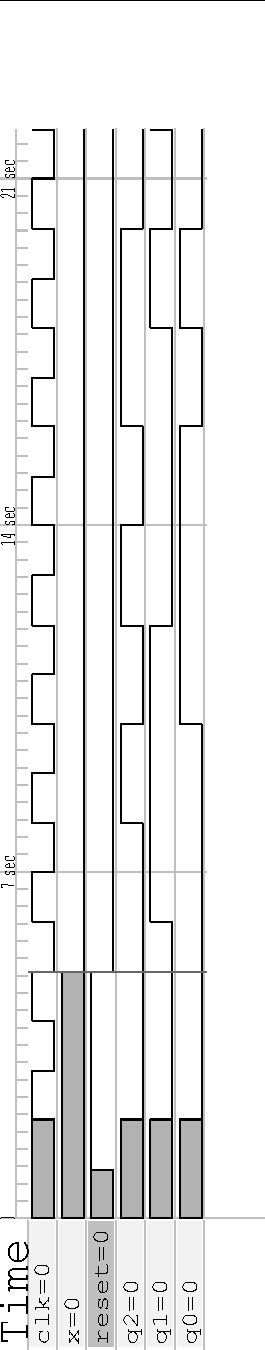
\includegraphics[angle=-90,scale=0.7]{verilog/3bitcounter-up}
(a)
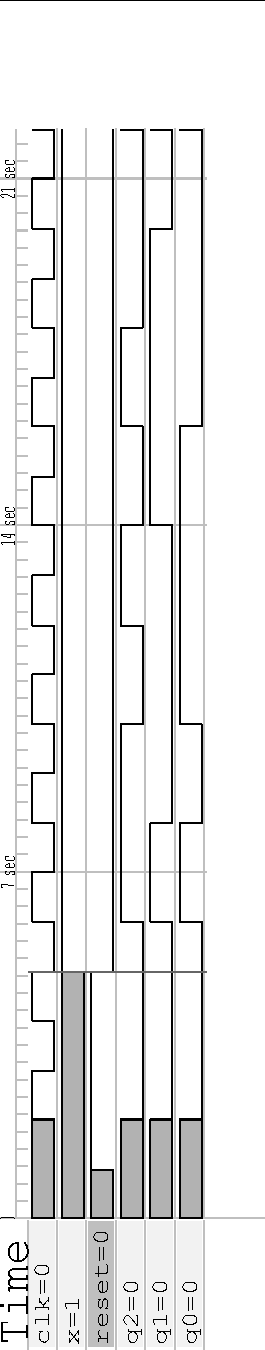
\includegraphics[angle=-90,scale=0.7]{verilog/3bitcounter-down}
(b)
\caption{Output of GTKWave when counting up (a) ($X = 0$) and
down (b) ($X = 1$).}
\label{fig:wave}
\end{figure}

The output of GTKWave for a counting sequence going up with
a reset in the middle is given in Figure \ref{fig:wavereset}.
The outputs are reset to zero and it resumes counting up with
the next value of 0 1 0 as it should.

\begin{figure}
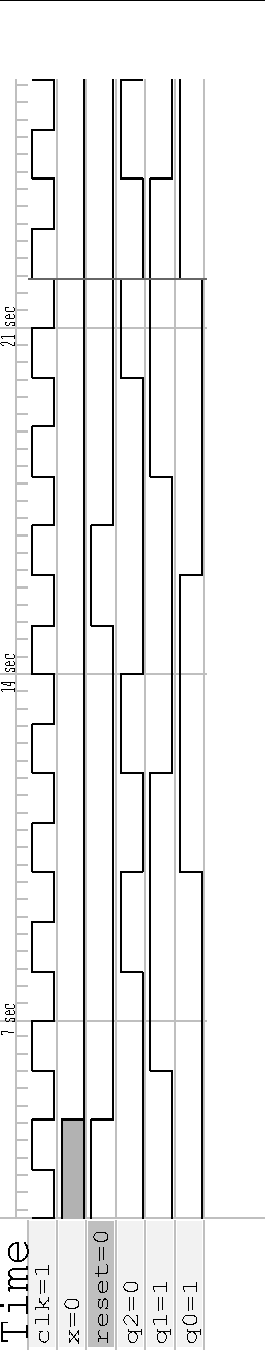
\includegraphics[angle=-90,scale=0.7]{verilog/3bitcounter-reset}
\caption{Output of GTKWave for the reset condition in the middle
of a counting sequence.}
\label{fig:wavereset}
\end{figure}

% }}}

% {{{ Conclusion
\section{Conclusion}

This lab was a complete success in implementing a three bit non-sequential
counter with a synchronous reset in Verilog.
All design requirements were met and the counter behaved as
expected.

% }}}

%\clearpage

\renewcommand*{\refname}{\vspace{-8mm}}
\section{References}
%%\bibliographystyle{plain}
%%\bibliographystyle{mslapa}
\bibliographystyle{ieeetr}
\bibliography{../references}

\appendix

\clearpage
\section{Verilog Test Bench}
\label{sec:test}

\lstinputlisting[
	language=Verilog,
	basicstyle=\footnotesize,
	numbers=left
	]{verilog/test.v}


\end{document}

% vim:foldmethod=marker
